\documentclass[10pt, letterpaper]{article}

% Packages:
\usepackage[
    ignoreheadfoot,
    top=2 cm,
    bottom=2 cm,
    left=2 cm,
    right=2 cm,
    footskip=1.0 cm,
    % showframe
]{geometry}
\usepackage{titlesec}
\usepackage{tabularx}
\usepackage{array}
\usepackage[dvipsnames]{xcolor}
\definecolor{primaryColor}{RGB}{0, 79, 144}
\usepackage{enumitem}
\usepackage{fontawesome5}
\usepackage{amsmath}
\usepackage{graphicx}
\usepackage[
    pdftitle={Jongyun Hur's CV},
    pdfauthor={Jongyun Hur},
    pdfcreator={LaTeX with RenderCV},
    colorlinks=true,
    urlcolor=primaryColor
]{hyperref}
\usepackage[pscoord]{eso-pic}
\usepackage{calc}
\usepackage{bookmark}
\usepackage{lastpage}
\usepackage{changepage}
\usepackage{paracol}
\usepackage{ifthen}
\usepackage{needspace}
\usepackage{iftex}
\usepackage{etoolbox}

% Ensure that generated PDF is machine readable:
\ifPDFTeX
    \input{glyphtounicode}
    \pdfgentounicode=1
    % \usepackage[T1]{fontenc}
    \usepackage[utf8]{inputenc}
    \usepackage{lmodern}
\fi

% General settings:
\AtBeginEnvironment{adjustwidth}{\partopsep0pt}
\pagestyle{empty}
\setcounter{secnumdepth}{0}
\setlength{\parindent}{0pt}
\setlength{\topskip}{0pt}
\setlength{\columnsep}{0cm}

% Footer:
\makeatletter
\let\ps@customFooterStyle\ps@plain
\patchcmd{\ps@customFooterStyle}{\thepage}{
    \color{gray}\textit{\small Jongyun Hur - Page \thepage{} of \pageref*{LastPage}}
}{}{}
\makeatother
\pagestyle{customFooterStyle}

% Section formatting:
\titleformat{\section}
    {\needspace{4\baselineskip}\bfseries\large}
    {}
    {0pt}
    {}
    [\vspace{1pt}\titlerule]

\titlespacing{\section}{
    -1pt
}{
    0.3 cm
}{
    0.2 cm
}

% Bullet formatting:
\renewcommand\labelitemi{$\circ$}

\newenvironment{highlights}{
    \begin{itemize}[
        topsep=0.10 cm,
        parsep=0.10 cm,
        partopsep=0pt,
        itemsep=0pt,
        leftmargin=0.4 cm + 10pt
    ]
}{
    \end{itemize}
}

\newenvironment{highlightsforbulletentries}{
    \begin{itemize}[
        topsep=0.10 cm,
        parsep=0.10 cm,
        partopsep=0pt,
        itemsep=0pt,
        leftmargin=10pt
    ]
}{
    \end{itemize}
}

% One-column entry:
\newenvironment{onecolentry}{
    \begin{adjustwidth}{
        0.2 cm + 0.00001 cm
    }{
        0.2 cm + 0.00001 cm
    }
}{
    \end{adjustwidth}
}

% Two-column entry:
\newenvironment{twocolentry}[2][]{
    \onecolentry
    \def\secondColumn{#2}
    \setcolumnwidth{\fill, 4.5 cm}
    \begin{paracol}{2}
}{
    \switchcolumn
    \raggedleft
    \secondColumn
    \end{paracol}
    \endonecolentry
}

% Header:
\newenvironment{header}{
    \setlength{\topsep}{0pt}\par\kern\topsep
}{
    \par\kern\topsep
}

% Last updated text:
\newcommand{\placelastupdatedtext}{
    \AddToShipoutPictureFG*{
        \put(
            \LenToUnit{\paperwidth-2 cm-0.2 cm+0.05cm},
            \LenToUnit{\paperheight-1.0 cm}
        ){
            \vtop{
                {\null}
                \makebox[0pt][c]{
                    \small\color{gray}
                    \textit{Last updated in November 2026}
                    \hspace{\widthof{Last updated in November 2026}}
                }
            }
        }
    }
}

% Save the original href command:
\let\hrefWithoutArrow\href

% External links:
\renewcommand{\href}[2]{
    \hrefWithoutArrow{#1}{
        \ifthenelse{\equal{#2}{}}{ }{#2 }
        \raisebox{.15ex}{\footnotesize \faExternalLink*}
    }
}

\begin{document}

    \newcommand{\AND}{\unskip
        \cleaders\copy\ANDbox\hskip\wd\ANDbox
        \ignorespaces
    }
    \newsavebox\ANDbox
    \sbox\ANDbox{}

    \setlength{\fboxsep}{1pt}
    \setlength{\fboxrule}{1pt}

    \placelastupdatedtext

    % =====================================================
    % Header: name above, text on the left, photo on the right
    % =====================================================

    \begin{header}

        {\centering
            \textbf{\fontsize{22pt}{26pt}\selectfont Jongyun Hur}
            \par
        }

        \vspace{0.3cm}

        \noindent
        \begin{minipage}[t]{0.74\textwidth}
            \vspace{0pt}

            \normalsize
            \mbox{%
                \hrefWithoutArrow{mailto:jongyun.jh@gmail.com}{%
                    \color{black}
                    {\footnotesize\faEnvelope[regular]}
                    \hspace*{0.13cm}jongyun.jh@gmail.com
                }%
            }

            \vspace{0.12cm}

            \mbox{%
                {\color{black}\footnotesize\faMapMarker*}
                \hspace*{0.13cm}Seoul, South Korea
            }

            \section{Research Interests}

            My primary research interest lies in computer architecture
            and hardware-software co-design for emerging computing
            systems. I enjoy exploring how hardware and software work
            together to create next-generation architectures and
            hardware accelerators. My goal is to enhance system
            efficiency and minimize energy consumption through
            effective hardware-software optimization.

        \end{minipage}%
        \hfill
        \begin{minipage}[t]{0.23\textwidth}
            \vspace{0pt}
            \raggedleft
            \fbox{%
                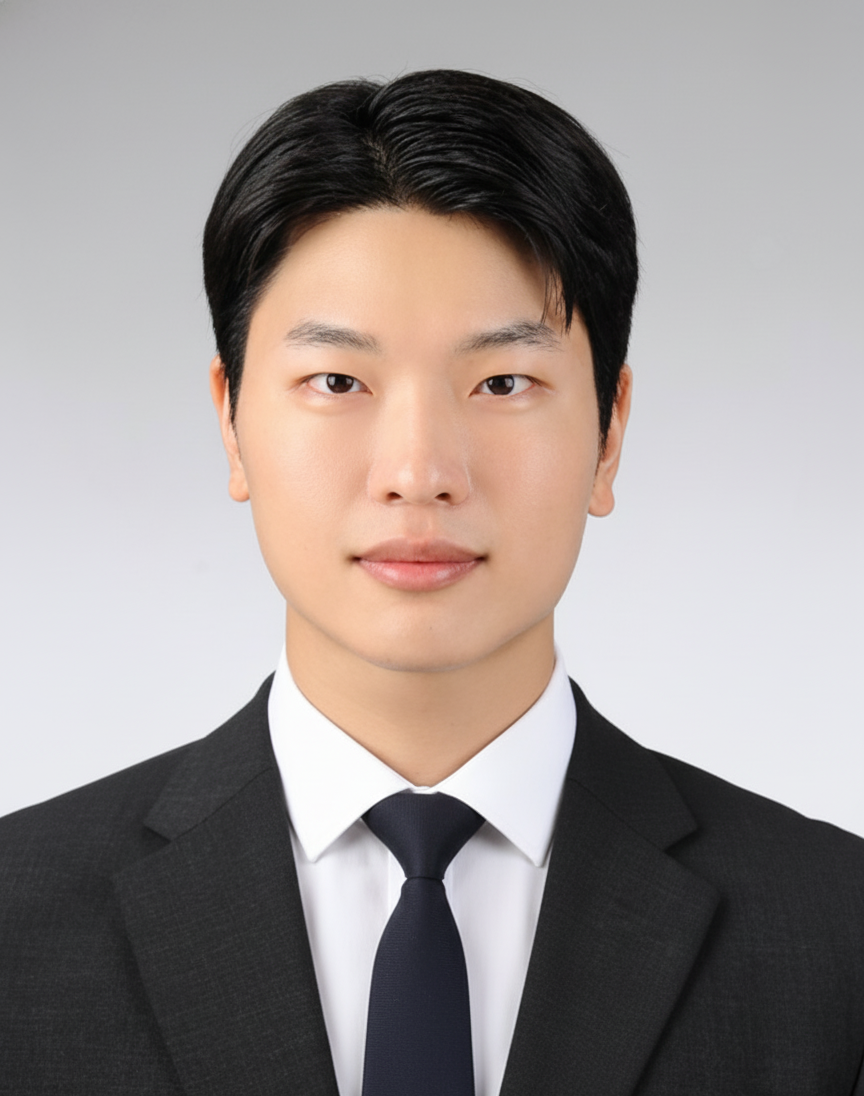
\includegraphics[
                    width=3.5cm,
                    height=4.5cm,
                    keepaspectratio
                ]{../assets/img/jongyun-hur-portrait.png}%
            }
        \end{minipage}

    \end{header}

    \vspace{0.1cm}

    % =====================================================
    % Education
    % =====================================================

    \section{Education}

        \begin{onecolentry}
            \textbf{Soongsil University}
            \hfill
            \textit{Seoul, South Korea}
            \\
            \textit{B.S. in Artificial Intelligence Software}
            \hfill
            \textit{Mar. 2022 -- Feb. 2028 (Expected)}
        \end{onecolentry}

        \vspace{0.10cm}

        \begin{onecolentry}
            \begin{highlights}
                \item \textbf{GPA:} Total 3.79/4.5, Major 3.78/4.5
                (106.5/133 credits)
            \end{highlights}
        \end{onecolentry}

    % =====================================================
    % Publications
    % =====================================================

    \section{Publications}

        \begin{onecolentry}
            \textbf{Jongyun Hur}, Seongheum Kim.
            ``Evaluating Latent-Space Mixture-of-Experts in Small
            Vision-Language Models.''
            \textit{Annual Conference of Korea Information Processing
            Society (ACK)}, 2026.
        \end{onecolentry}

    % =====================================================
    % Internship
    % =====================================================

    \section{Internship}

        \begin{twocolentry}{
            \textit{Ulsan, South Korea}
            \\
            \textit{Jan. 2026 -- Feb. 2026}
        }
            \textbf{UNIST (Ulsan National Institute of Science and Technology)}
            \\
            \text{Undergraduate Research Intern, CoCoLab (Advisor: Prof. Ranggi Hwang)}
        \end{twocolentry}

        \vspace{0.10 cm}

        \begin{onecolentry}
            \begin{highlights}
                \item \textbf{Developed a cycle-level hardware simulator
                for Sparse CNNs (SCNN)} to accurately model Cartesian
                product-based sparse convolution and its unique dataflow.

                \item Identified architectural bottlenecks by evaluating
                key performance metrics, including multiplier utilization,
                PE idle cycles, accumulator bank conflicts, and
                queue-induced pipeline stalls.
            \end{highlights}
        \end{onecolentry}

        \vspace{0.4 cm}

        \begin{twocolentry}{
            \textit{Seoul, South Korea}
            \\
            \textit{Aug. 2025 -- Nov. 2025}
        }
            \textbf{Potatonet}
            \\
            \text{Machine Learning Engineer Intern}
        \end{twocolentry}

        \vspace{0.10 cm}

        \begin{onecolentry}
            \begin{highlights}
                \item \textbf{Reworked frame selection} for electric
                vehicle fire detection, using a lightweight detector
                to identify smoke and flame candidates and select
                recent frames based on detection confidence and
                capture time.

                \item \textbf{Implemented bounded buffering and
                selective preprocessing} to limit stale-frame
                accumulation and redundant inference with
                Qwen2.5-VL-3B on Jetson Orin Nano.
            \end{highlights}
        \end{onecolentry}

        \vspace{0.2 cm}

    % =====================================================
    % Awards
    % =====================================================

    \section{Awards}

        \begin{onecolentry}
            \begin{highlights}
                \item \textbf{President's Award (1st Place)},
                Soongsil University AI Software Competition
                \hfill
                \textit{Jul. 2026}

                \item \textbf{3rd Place},
                2026 Pre-Startup Team \& Startup Club Discovery Hackathon
                \hfill
                \textit{May 2026}

                \item \textbf{2nd Place},
                Soongsil University AI Convergence Competition
                \hfill
                \textit{Nov. 2023}
            \end{highlights}
        \end{onecolentry}

    % =====================================================
    % Language Proficiency
    % =====================================================

    \section{Language Proficiency}

        \begin{onecolentry}
            \begin{highlights}
                \item TOEFL iBT: 4.5/6.0 (Comparable Score: 90/120)
                \hfill
                \textit{Sep. 2026}
            \end{highlights}
        \end{onecolentry}

\end{document}
